\subsubsection{A familiar strategy}\seclabel{familiar}

We can also use the strategy $H^*_{\psi; K}$ of \cite{finding-adam}
and \secref{heart-upper} to get all the nodes of $S$; in this section,
when the procedure is used to find all nodes of the seed, we omit the
asterisk for notational consistency. More specifically, we study the
smallest choice of $K$ for which $H_{\psi; K}$ contains all nodes of
$S$ with probability at least $1 - \eps$, and such a choice will give
an upper bound on $K(k, \ell, \eps)$.

If $\psi(u) = |(T, u)_{v \downarrow}|$ for $v$ adjacent to $u$, we
will say that $\psi(u)$ is \emph{witnessed at $v$}.

\begin{prop}\proplabel{whole-upper}
  There are universal constants $c, \eps_0 > 0$ such that, if
  $\eps \le \eps_0$ and 
  \[
    K \ge (c k \ell/\eps) \log (k \ell/\eps) ,
  \]
  then
  \[
    \Pr\{V(S) \subseteq H_{\psi; K}(T^\circ)\} \ge 1 - \eps .
  \]
\end{prop}
\begin{proof}
  \begin{figure}
    \centering
    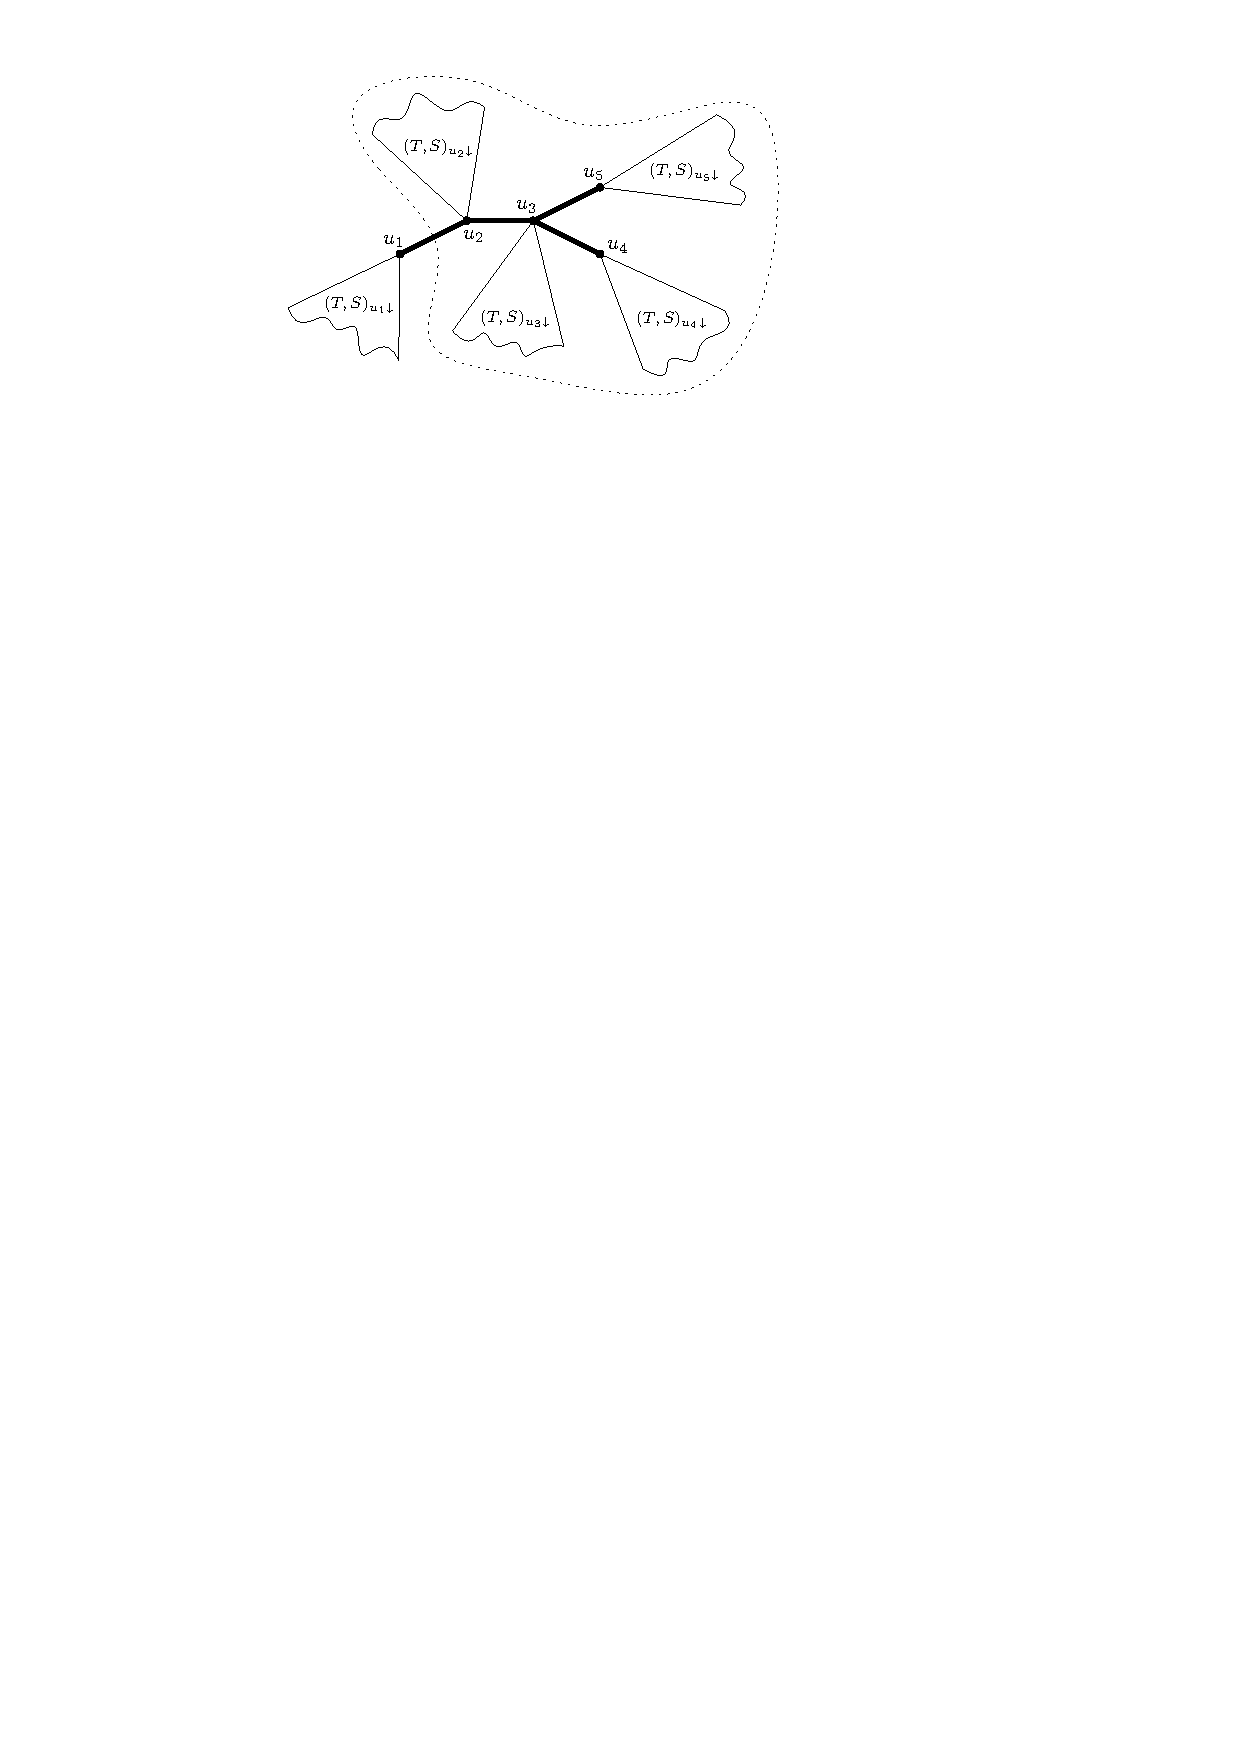
\includegraphics[width=0.6\textwidth]{witness.pdf}
    \caption{The seed $S$ has vertex set $\{u_1, \dots,
      u_5\}$. Suppose that $\psi^* = \psi(u_1)$. Then, $\psi^*$ is
      witnessed at $u_2$, and $\psi^*$ correponds to the size of the
      outlined subgraph.}
    \figlabel{whole-upper}
  \end{figure}
  The proof is similar to that of \propref{heart-upper}. Write
  \[
    \psi^* = \max\{\psi(u_1), \dots, \psi(u_k)\} .
  \]
  Observe that if for all $i > K$, $\psi(u_i) > \psi^*$, then
  $V(S) \subseteq H_{\psi; K}(T^\circ)$. So,
  \begin{equation}
    \Pr\{V(S) \not\subseteq H_{\psi; K}(T^\circ)\} \le \Pr\{\psi^* \ge n t \} + \Pr\{\exists i > K \colon \psi(u_i) \le n t\} \eqlabel{phi-tail-whole}
  \end{equation}
  for $t > 0$ to be specified. We handle the first term in
  \eqref{phi-tail-whole}: Suppose that $\psi^*$ is attained by
  $u \in V(S)$ and witnessed by its child $v \not\in V(S)$, \ie
  \[
    \psi^* = \psi(u) = |(T, u)_{v \downarrow}| ,
  \]
  Then, $u$ has a neighbour $w \in V(S)$, and
  \[
    \psi(w) \ge |(T, w)_{u \downarrow}| > |(T, u)_{v \downarrow}| = \psi(u) ,
  \]
  so $\psi(u)$ cannot be maximum. Thus, $\psi^*$ must be witnessed by
  a node of $V(S)$, and in particular, one can iterate the above
  motion to see that $\psi^*$ must be attained by a leaf of $S$ and
  witnessed by its unique neighbour in $S$, so
  \[
    \psi^* = \max_{u \in L(S)} \sum_{v \in V(S) - u} |(T, S)_{v \downarrow}| .
  \]
  See \figref{whole-upper} for an illustration. By
  \lemref{dir-convergence}, for any $u \in L(S)$,
  \[
    \frac{1}{n} \sum_{v \in V(S) - u} |(T, S)_{v \downarrow}| \overset{d}{\to} \Beta(k - 1, 1) ,
  \]
  as $n \to \infty$, so
  \begin{align*}
    \Pr\{\psi^* \ge nt\} &\le \Pr\left\{\exists u \in L(S) \colon \sum_{v \in V(S) - u} |(T, S)_{v \downarrow}| \ge n t \right\} \\
                         &\le \ell \Pr\{\Beta(k - 1, 1) \ge t\} \\
                         &= \ell (1 - t^{k - 1}) .
  \end{align*}
  We can make this at most $\eps/2$ by choosing
  $t = (1 - \eps/(2\ell))^{1/(k - 1)}$.

  For the second term in \eqref{phi-tail-whole}, the argument is again
  identical to that of \cite[Theorem 3]{finding-adam}, and we can say
  that
  \begin{align*}
    \Pr\{\exists i > K \colon \psi(u_i) \le nt\} \le K t^{K - 1} \le K e^{-\frac{\eps (K - 1)}{2 (k - 1)\ell}} .
  \end{align*}
  Picking $K \ge (c k \ell/\eps) \log (k\ell/\eps)$ for some constant
  $c > 0$ gives the desired result, as long as $\eps \le \eps_0$ for
  some constant $\eps_0 > 0$.
\end{proof}
Again, the set $H_{\psi; K}(T^\circ)$ can be computed in $O(n)$
time. We show in \lemref{leaf-existence} that the result of
\thmref{whole-upper} involves the right order for $K$ for the strategy
given by $H_{\psi; K}$, up to logarithmic factors: When
$K \le k \ell/(4 \eps)$, then with probability at least $\eps$, at
least one leaf of $S$ is also a leaf of $T \sim \UA(K, S)$, and any
leaf of $T$ maximizes the value of $\psi$.

\subsubsection{A reduction to intersection testing}

We now consider an alternative procedure for locating all nodes of the
seed, which sometimes requires fewer nodes than $H_{\psi; K}$ to
succeed with probability $1 - \eps$. We define the set
$H_{\phi; K, k, \ell, \eps}(T^\circ)$ as follows:
\begin{enumerate}[label=(\roman*)]
\item Let $H^*$ be a set of size $K^*(k, \ell, \eps/2)$ which
  intersects the seed with probability at least $1 - \eps/2$;
\item For each $u \in H^*$, traverse the tree $T$ in a depth-first
  manner around $u$;
\item When exploring $v \in T$, add $v$ to
  $H_{\phi; K, k, \ell, \eps}(T^\circ)$ if
  $|(T, u)_{v \downarrow}| \ge n\eps/(2 k\ell)$, and stop exploring
  this path otherwise. Stop at any point if the size of the set
  exceeds $K$.
\end{enumerate}
If we can prove that $H_{\phi; K, k, \ell, \eps}(T^\circ)$ includes
the whole seed with probability at least $1 - \eps$, and that $K$ is
sufficiently large, we obtain an upper bound on $K(k, \ell, \eps)$.
\begin{prop}\proplabel{whole-upper-ez}
  If $K \ge (2k \ell/\eps) K^*(k, \ell, \eps/2)$, then
  \[
    \Pr\{V(S) \subseteq H_{\phi; K, k, \ell, \eps}(T^\circ)\} \ge 1 -
    \eps .
  \]
\end{prop}
\begin{proof}
  We show the failure probability is small enough:
  \begin{align*}
    \Pr\{V(S) \not\subseteq H_{\phi; K, k, \ell, \eps}(T^\circ)\} \le \Pr\biggl\{V(S) \cap H^* = \emptyset\biggr\} + \Pr\biggl\{\min_{u \in L(S)} |(T, S)_{u \downarrow}| < \frac{n\eps}{2 k \ell}\biggr\} .
  \end{align*}
  The first term is at most $\eps/2$ by definition. For the second
  term, note that
  \[
    \frac{\min_{u \in L(S)} |(T, S)_{u \downarrow}|}{n} \overset{d}{\to} \frac{\Beta(1, k - 1)}{\ell} ,
  \]
  as $n \to \infty$ by \lemref{sukhatme}, so
  \begin{align*}
    \Pr\biggl\{\min_{u \in L(S)} |(T, S)_{u \downarrow}| < \frac{n \eps}{2k \ell}\biggr\} &\le \Pr\biggl\{\Beta(1, k - 1) \le \frac{\eps}{2k}\biggr\} \\
                                                                      &= 1 - \left(1 - \frac{\eps/2}{k}\right)^{k - 1} \\
                                                                                 &\le 1 - e^{-\eps/2} \\
                                                                                 &\le \eps/2 ,
  \end{align*}
  as desired. Finally, for $u$ fixed, there are at most
  $2 k \ell/\eps$ nodes $v$ such that
  $|(T, u)_{v \downarrow}| \ge n\eps/(2k\ell)$, so $K$ is indeed large
  enough to include all desired nodes.
\end{proof}
By a remark in \secref{mle}, the set $H^*$ in the above construction
can be computed in polynomial time, so
$H_{\phi; K, k, \ell, \eps}(T^\circ)$ can be computed in polynomial
time. \thmref{whole-upper} follows immediately from
\propref{whole-upper} and \propref{whole-upper-ez}.
